\section{The User Interface ("`ui2user"')}
This section specifies the appereance of the user interface to the user.

% Nico: 1.0
%---------------------------------------------------------------------
\subsection{Interface}
The UI is running as a ncurses application and prompts for input
on a specific line.\footnote{Example output can be found in figure \ref{startup}.}
All commands start with "/".
\begin{figure}[h]
    \caption{UI Startup Screen}
    \label{startup}
    \centering
    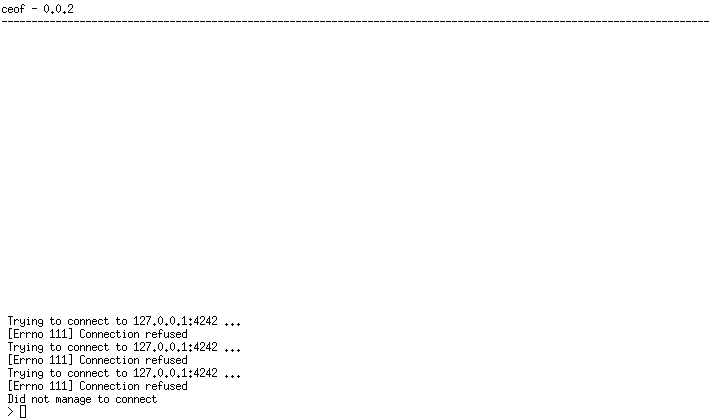
\includegraphics[width=10cm]{ui-startup.png}
\end{figure}

%---------------------------------------------------------------------
\subsection{UI Command: /help}
The /help command prints a short usage
description.\footnote{Example output can be found in figure \ref{help}.}

\subsubsection{Example}
\begin{verbatim}
/help
\end{verbatim}
% /connect [host] [port] - Connect to chat server
% /quit - Quit this UI
% /allquit - Quit this UI, Chatserver and all other UIs
% /peer add <name> <address> <keyid> - Add peer
% /peer del <name> - Delete peer
% /peer send <name> <message> - Send message to peer
% /peer rename <oldname> <newname> - Rename peer
% /peer show <name> - Show peer
% /peer list - List all peers
\begin{figure}[h]
    \caption{UI Help Output}
    \label{help}
    \centering
    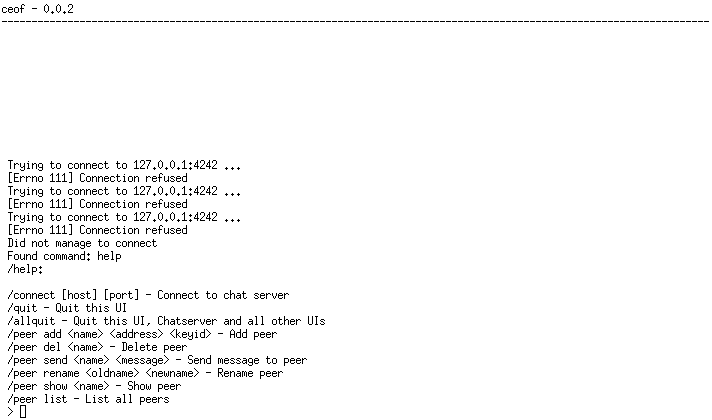
\includegraphics[width=10cm]{help-command.png}
\end{figure}

%---------------------------------------------------------------------
\subsection{UI Command: /connect $[$host$]$ $[$port$]$}
The connect command can be used to connect to the chat
server.\footnote{Example output can be found in figure \ref{connect}.}
Host and port are optional. If omitted, the saved host and/or
port will be used. This command uses message 2100.
\begin{figure}[h]
    \caption{UI /connect}
    \label{connect}
    \centering
    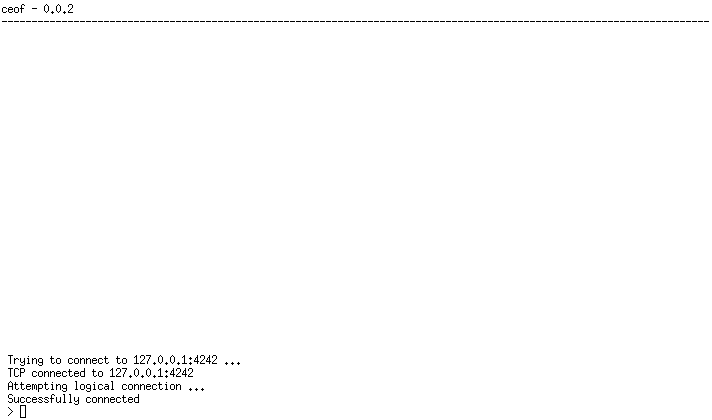
\includegraphics[width=10cm]{connected-to-cs.png}
\end{figure}

\subsubsection{Example}
\begin{verbatim}
/connect 127.0.0.1 4242
\end{verbatim}
% Nico: Code & Doc
%---------------------------------------------------------------------
\subsection{UI Command: /quit}
Request the user interface to exit. It will deregister from the CS.
This command uses message 2101.
\subsubsection{Example}
\begin{verbatim}
/quit
\end{verbatim}
% Nico: 1.0
%---------------------------------------------------------------------
\subsection{UI Command: /allquit}
The UI tells the CS and all connected UIs (including itself) to quit.
This command uses message 2199.\footnote{Example output can be found in figure \ref{allquit}.}
\begin{figure}[h]
    \caption{UI /allquit}
    \label{allquit}
    \centering
    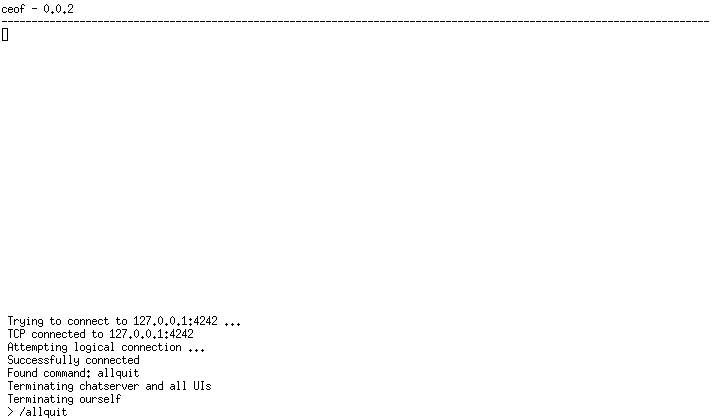
\includegraphics[width=10cm]{allquit.png}
\end{figure}

\subsubsection{Example}
\begin{verbatim}
/allquit
\end{verbatim}
% Nico: 1.0
%---------------------------------------------------------------------
\subsection{UI Command: /peer add $<$name$>$ $<$address$>$ $<$keyid$>$}
Add the peer with the given name \textit{name} to the list
of known peers.\footnote{Example output can be found in figure \ref{peeradd}.}
\begin{figure}[h]
    \caption{UI /peer add}
    \label{peeradd}
    \centering
    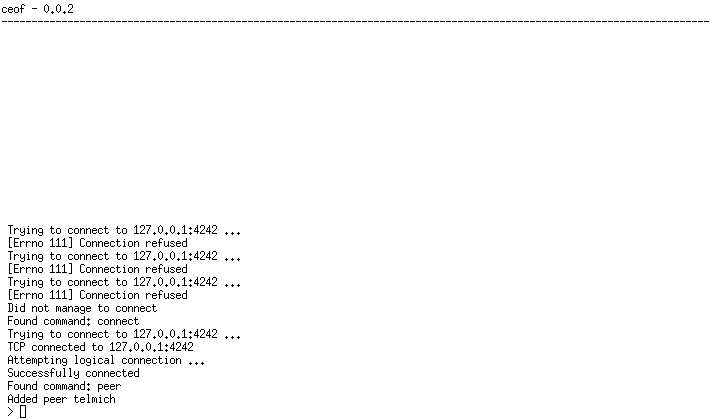
\includegraphics[width=10cm]{peer-add.png}
\end{figure}


\index{UI Command!/peer add}%
\begin{longtable}{|c|c|c|c|}
\caption{UI Command: /peer add parameters}\\
\hline
\textbf{Parameter} & \textbf{Type} & \textbf{Description} & \textbf{Example}\\
\hline
Peer name & EOFsdt: name & Name you identify the peer with & telmich\\
\hline
Address & EOFsdt: address & Where we can make the first contact & tcp://10.0.42.42:4242\\
\hline
Keyid & EOFsdt: keyid & The PGP fingerprint of the peers public key & F27987E34E66...\\
\hline
\end{longtable}

\subsubsection{Example}
\begin{verbatim}
/peer add telmich tcp//:10.0.42.42:4242 F27987E34E7866B2BA39C2FD793EB8FC325251FE
\end{verbatim}
% Nico: 1.0
%---------------------------------------------------------------------
\subsection{UI Command: /peer del $<$name$>$}
Delete the peer with the given name \textit{name} from the list of
known peers.\footnote{Example output can be found in figure \ref{peerdel}.}
\begin{figure}[h]
    \caption{UI /peer del}
    \label{peerdel}
    \centering
    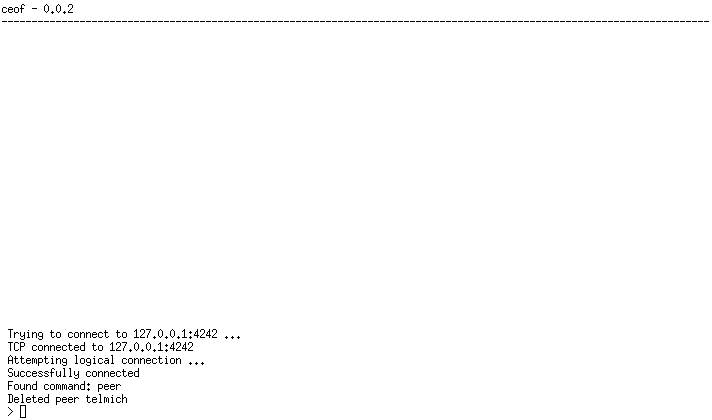
\includegraphics[width=10cm]{peer-del.png}
\end{figure}


\index{UI Command!/peer del}%
\begin{longtable}{|c|c|c|c|}
\caption{UI Command: /peer del parameters}\\
\hline
\textbf{Parameter} & \textbf{Type} & \textbf{Description} & \textbf{Example}\\
\hline
Peer name & EOFsdt: name & Name you identify the peer with & telmich\\
\hline
\end{longtable}

\subsubsection{Example}
\begin{verbatim}
/peer del telmich
\end{verbatim}
% Nico: 1.0
%---------------------------------------------------------------------
\subsection{UI Command: /peer send $<$name$>$ $<$msgtext$>$}
Send message \textit{msgtext} to peer
\textit{name}.\footnote{Example output can be found in figure \ref{peersend}.}
\begin{figure}[h]
    \caption{UI /peer send}
    \label{peersend}
    \centering
    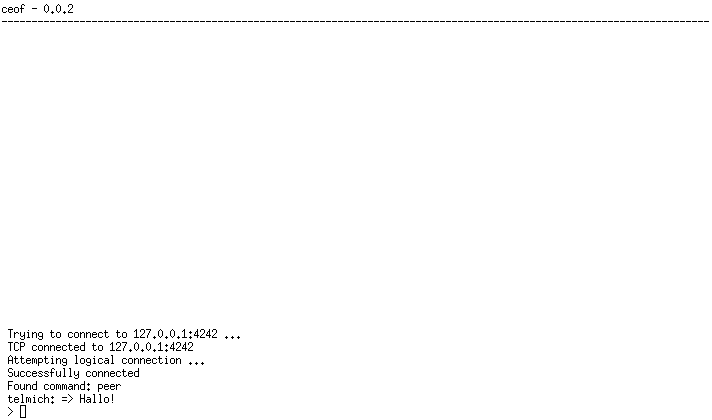
\includegraphics[width=10cm]{peer-send.png}
\end{figure}


\index{UI Command!/peer send}%
\begin{longtable}{|c|c|c|c|}
\caption{UI Command: /peer send parameters}\\
\hline
\textbf{Parameter} & \textbf{Type} & \textbf{Description} & \textbf{Example}\\
\hline
Name & EOFsdt: name & Name you identify the peer with & telmich\\
\hline
Msgtext & EOFsdt: msgtxt & The message itself & Hallo, wie geht es Dir?\\
\hline
\end{longtable}

\subsubsection{Example}
\begin{verbatim}
/peer send telmich Hallo, wie geht es Dir?
\end{verbatim}
% Nico: 1.0
%---------------------------------------------------------------------
\subsection{UI Command: /peer rename $<$oldname$>$ $<$newname$>$}
Renames the peer.\footnote{Example output can be found in figure \ref{peerrename}.}
\begin{figure}[h]
    \caption{UI /peer rename}
    \label{peerrename}
    \centering
    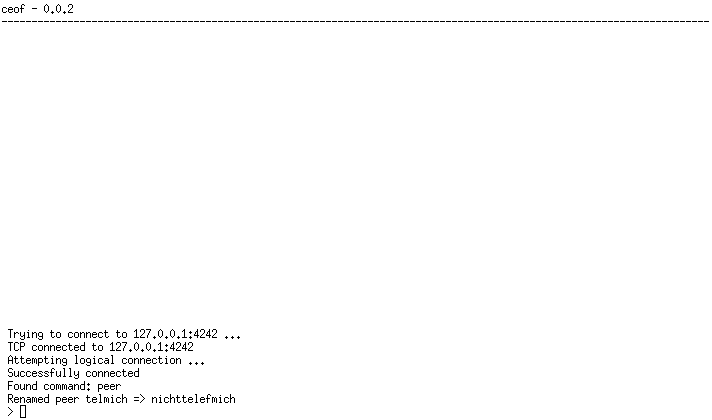
\includegraphics[width=10cm]{peer-rename.png}
\end{figure}


\index{UI Command!/peer rename}%
\begin{longtable}{|c|c|c|c|}
\caption{UI Command: /peer rename parameters}\\
\hline
\textbf{Parameter} & \textbf{Type} & \textbf{Description} & \textbf{Example}\\
\hline
Oldname & EOFsdt: name & Old name & susi\\
\hline
Newname & EOFsdt: name & New name & heinz\\
\hline
\end{longtable}

\subsubsection{Example}
\begin{verbatim}
/peer rename susi heinz
\end{verbatim}
% Nico: 1.0
%---------------------------------------------------------------------
\subsection{UI Command: /peer show $<$name$>$}
Display detailled information about peer.\footnote{Example output can be found in figure \ref{peershow}.}
\begin{figure}[h]
    \caption{UI /peer show}
    \label{peershow}
    \centering
    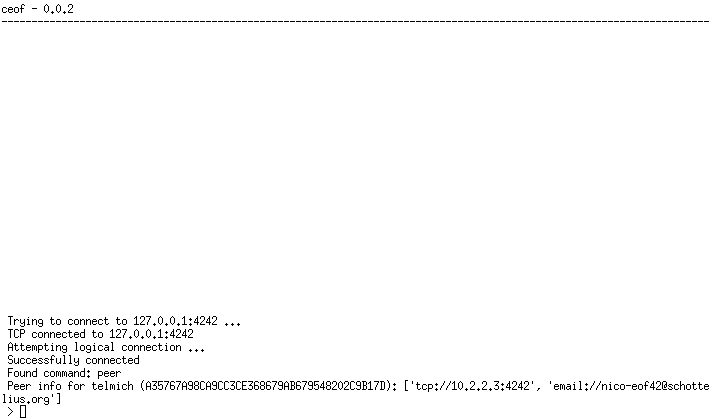
\includegraphics[width=10cm]{peer-show.png}
\end{figure}

\index{UI Command!/peer show}%
\begin{longtable}{|c|c|c|c|}
\caption{UI Command: /peer rename parameters}\\
\hline
\textbf{Parameter} & \textbf{Type} & \textbf{Description} & \textbf{Example}\\
\hline
Peer name & EOFsdt: name & Name as known by CS & karl-otto\\
\hline
\end{longtable}

\subsubsection{Example}
\begin{verbatim}
/peer show karl-otto
\end{verbatim}
% Nico: 1.0
%---------------------------------------------------------------------
\subsection{UI Command: /peer list}
List of currently known peers. This command does not accept any
parameters.\footnote{Example output can be found in figure \ref{peerlist}.}
\begin{figure}[h]
    \caption{UI /peer list}
    \label{peerlist}
    \centering
    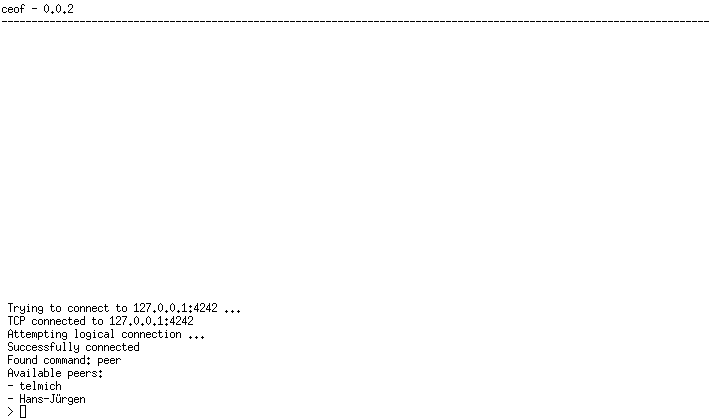
\includegraphics[width=10cm]{peer-list.png}
\end{figure}


\subsubsection{Example}
\begin{verbatim}
/peer list
\end{verbatim}
% Nico: 1.0
% %---------------------------------------------------------------------
% \subsection{Aliases}
% Aliases may optionally be provided by the UI. If an UI provides
% support for aliases, it must implement the "`\emph{/alias}"' command.
% 
% The following aliases should be provided by default,
% to aid new users using EOF.
% % Nico: 1.0
% %---------------------------------------------------------------------
% \subsection{/alias $<aliasname>$ $<command...>$}
% This command should be used to setup aliases.
% % Nico: 1.0
% %---------------------------------------------------------------------
% \subsection{/msg $<name>$ $<msgtext>$}
% Should be an alias for \textit{/peer send $<$name$>$ $<$msgtext$>$}
% % Nico: 1.0
% %---------------------------------------------------------------------
% \subsection{/whois $<name>$}
% Should be an alias for \textit{/peer show $<$name$>$}
% Nico: 1.0
